% Options for packages loaded elsewhere
\PassOptionsToPackage{unicode}{hyperref}
\PassOptionsToPackage{hyphens}{url}
%
\documentclass[12pt, letterpaper
]{article}
\usepackage{amsmath,amssymb}
\usepackage{lmodern}
\usepackage{iftex}
\ifPDFTeX
  \usepackage[T1]{fontenc}
  \usepackage[utf8]{inputenc}
  \usepackage{textcomp} % provide euro and other symbols
\else % if luatex or xetex
  \usepackage{unicode-math}
  \defaultfontfeatures{Scale=MatchLowercase}
  \defaultfontfeatures[\rmfamily]{Ligatures=TeX,Scale=1}
\fi
% Use upquote if available, for straight quotes in verbatim environments
\IfFileExists{upquote.sty}{\usepackage{upquote}}{}
\IfFileExists{microtype.sty}{% use microtype if available
  \usepackage[]{microtype}
  \UseMicrotypeSet[protrusion]{basicmath} % disable protrusion for tt fonts
}{}
\makeatletter
\@ifundefined{KOMAClassName}{% if non-KOMA class
  \IfFileExists{parskip.sty}{%
    \usepackage{parskip}
  }{% else
    \setlength{\parindent}{0pt}
    \setlength{\parskip}{6pt plus 2pt minus 1pt}}
}{% if KOMA class
  \KOMAoptions{parskip=half}}
\makeatother
\usepackage{xcolor}
\IfFileExists{xurl.sty}{\usepackage{xurl}}{} % add URL line breaks if available
\IfFileExists{bookmark.sty}{\usepackage{bookmark}}{\usepackage{hyperref}}
\hypersetup{
  hidelinks,
  pdfcreator={LaTeX via pandoc}}
\urlstyle{same} % disable monospaced font for URLs
\usepackage{graphicx}
\makeatletter
\def\maxwidth{\ifdim\Gin@nat@width>\linewidth\linewidth\else\Gin@nat@width\fi}
\def\maxheight{\ifdim\Gin@nat@height>\textheight\textheight\else\Gin@nat@height\fi}
\makeatother
% Scale images if necessary, so that they will not overflow the page
% margins by default, and it is still possible to overwrite the defaults
% using explicit options in \includegraphics[width, height, ...]{}
\setkeys{Gin}{width=\maxwidth,height=\maxheight,keepaspectratio}
% Set default figure placement to htbp
\makeatletter
\def\fps@figure{htbp}
\makeatother
\setlength{\emergencystretch}{3em} % prevent overfull lines
\providecommand{\tightlist}{%
  \setlength{\itemsep}{0pt}\setlength{\parskip}{0pt}}
\setcounter{secnumdepth}{-\maxdimen} % remove section numbering
\ifLuaTeX
  \usepackage{selnolig}  % disable illegal ligatures
\fi

\title{3DViewer v2.0}
\author{PutinBoyZ}
\date{August 2022}

\begin{document}

\begin{titlepage}
  \maketitle
\end{titlepage}  

\textbf{Introduction}

3DViewer\_v2.0 is a software designed to display .obj files. It lets the
user move, rotate and stretch the model and change display settings.

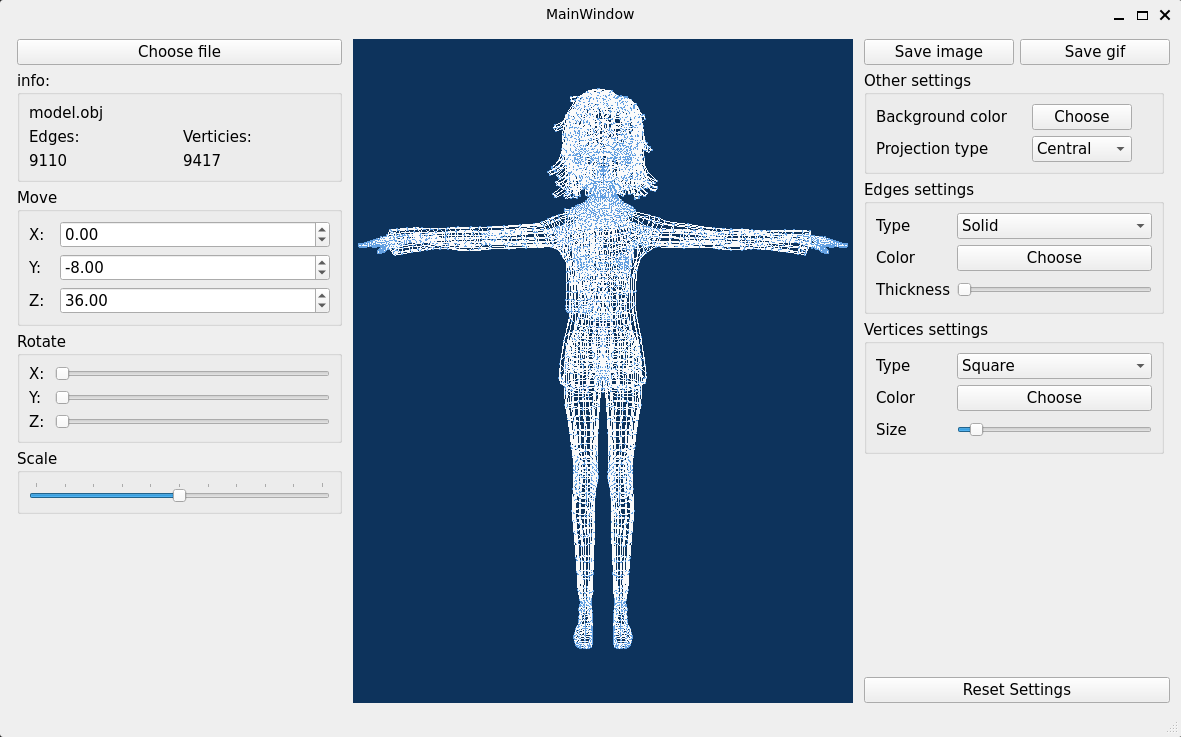
\includegraphics[width=4.72361in,height=2.94722in]{vertopal_4bce193b52fb40a8bfdc292270c39a64/media/image1.png}

\textbf{Features and capabilities}

The calculator supports three main modes of operation, including:

\begin{itemize}
\item
  Load and display complex wireframes without freezing the interface
\item
  Support for moving and rotating the model (including using the
  keyboard and mouse)
\item
  Display settings: choice of projection type, background color, color
  and style of vertices and edges
\item
  Saving images and animations
\end{itemize}

\textbf{Basics}

Using the "Choose file" button, open the model you are interested in.
After some time, the model will load (this may take some time, given the
size of the model and the performance of the computer). You can see a
summary of the model, move it, rotate it, and change the scale.

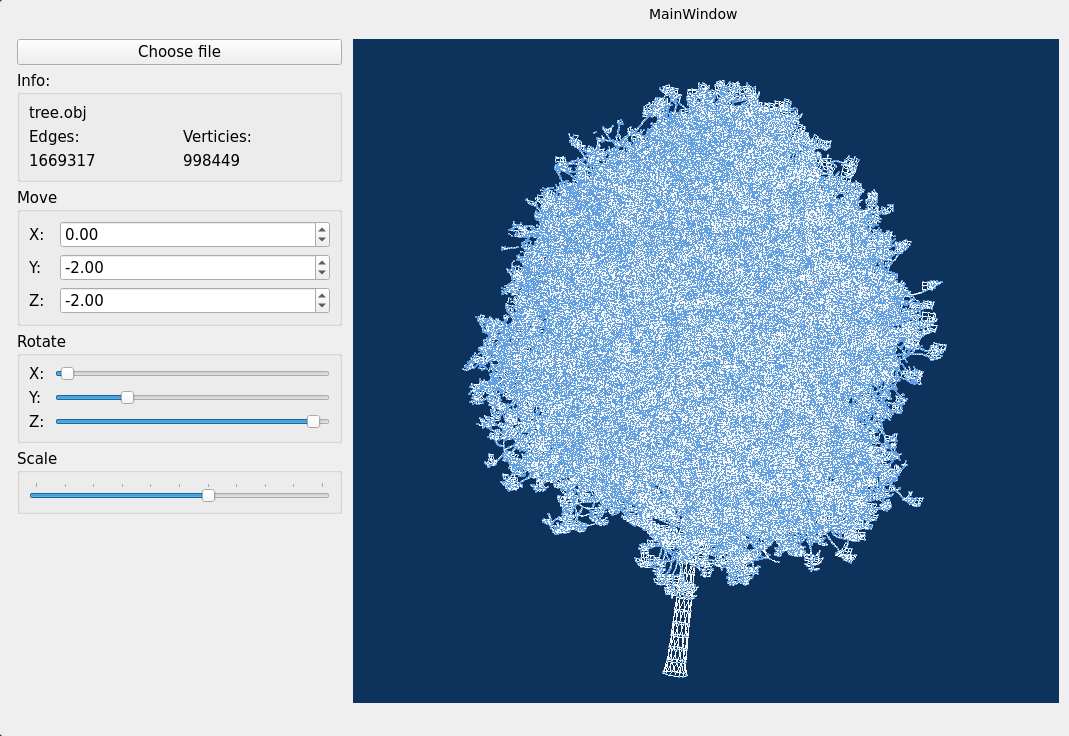
\includegraphics[width=4.72361in,height=3.25208in]{vertopal_4bce193b52fb40a8bfdc292270c39a64/media/image2.png}

You can also control the position of the model using the mouse or
keyboard:

\begin{itemize}
\item
  LMB --- model rotations by XY
\item
  RMB --- move along XY
\item
  WASD --- movement along XY
\item
  XZ --- movement along Z
\item
  QE --- rotation in Z
\item
  R --- position reset
\end{itemize}

\textbf{Styling}

Using the elements on the left, you can save an image or animation, set
model display settings, and reset them to default values.

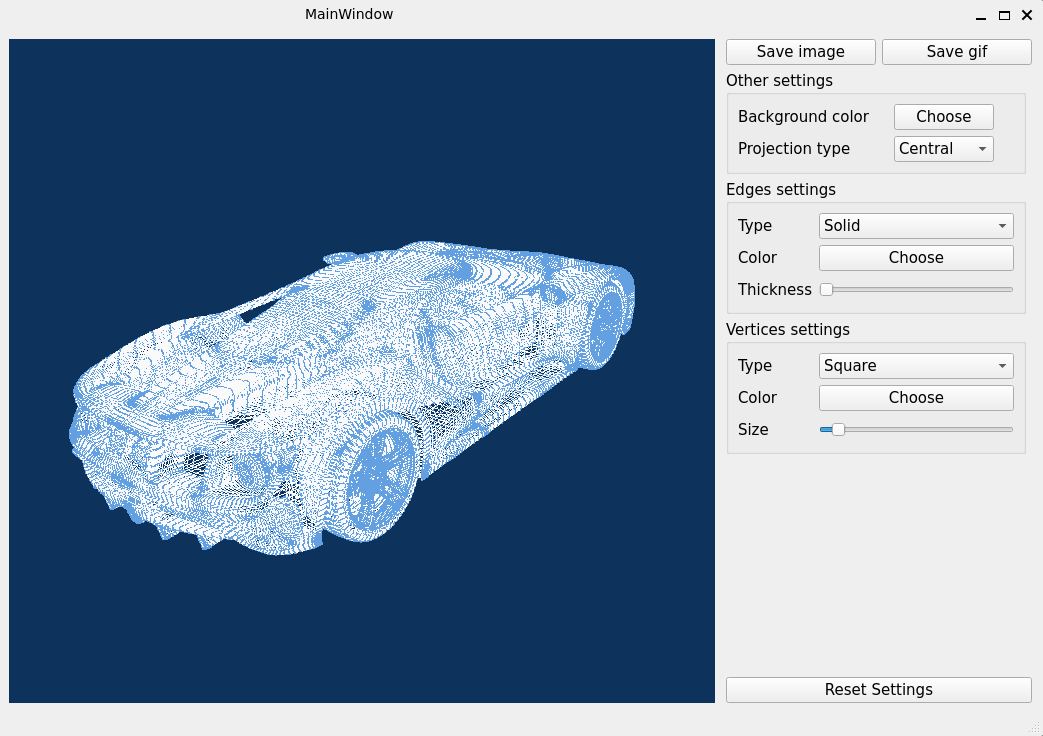
\includegraphics[width=4.72361in,height=3.33264in]{vertopal_4bce193b52fb40a8bfdc292270c39a64/media/image3.png}

\textbf{Usage}

Let's position the model and change the rendering settings a bit.

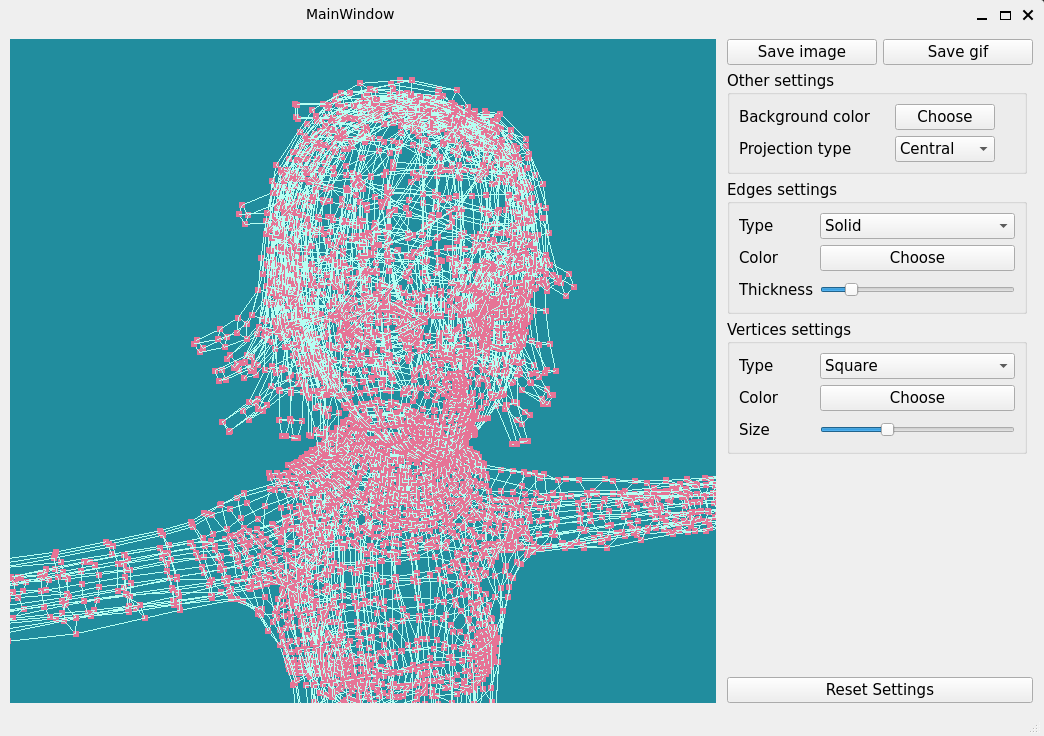
\includegraphics[width=4.72361in,height=3.32986in]{vertopal_4bce193b52fb40a8bfdc292270c39a64/media/image4.png}

\end{document}
